\documentclass[pstricks,14 pt]{extarticle}

	\usepackage[frenchb]{babel}
	\usepackage[utf8]{inputenc}  
	\usepackage[T1]{fontenc}
	\usepackage{amssymb}
	\usepackage[mathscr]{euscript}
	\usepackage{stmaryrd}
	\usepackage{amsmath}
	\usepackage{tabularx} 
	\usepackage{pstricks}
	\usepackage{pst-all} 
	\usepackage{tikz}
	\usepackage[all,cmtip]{xy}
	\usepackage{amsthm}
	\usepackage{varioref}
	\usepackage{geometry}
	\geometry{a4paper}
	\usepackage{lmodern}
	\usepackage{hyperref}
	\usepackage{array}
	 \usepackage{fancyhdr}
\usepackage{pstricks-add,multido}
	 \usepackage{float}
\renewcommand{\theenumi}{\alph{enumi})}
	\pagestyle{fancy}
	\theoremstyle{plain} 
	\fancyfoot[C]{} 
	\fancyhead[L]{Contrôle}
	\fancyhead[R]{Géométrie dans l'espace}\geometry{
 a4paper,
 total={170mm,257mm},
 left=10mm,
 top=18mm,
 bottom = 10mm
 }
	
	
	\title{Contrôle }
	\date{}
	\begin{document}
	{\begin{center}{\Large{Contrôle}}\end{center}}
\subsection*{Exercice 1 - 6 points}	%(1 + 2 + 2 + 1) 
Calculez le volume des figures suivantes, en centimètres cube. \begin{enumerate}
\item Un cube d'arête $5$ cm. 
\item Un pavé droit de largeur $2$ mm, de longueur $4$ dm et de hauteur $5$ mm. 
\item Un cône de rayon $2$ cm et de hauteur $3$ cm. (Donnez la formule exacte, puis la valeur approchée à l'unité en $\mathrm{cm}^3$.)
\item Une pyramide de hauteur $4$ cm et dont la base est un carré de côté $3$ cm. 

\end{enumerate}

\subsection*{Exercice 2 - 9 points}



\textbf{PARTIE A :} 6 points %=1+2+2+1

\medskip

Un magasin a reçu $650$ poissons dont $350$ poissons de type A et $300$ poissons de type B.

La responsable du magasin souhaite vendre ces poissons par lots de sorte que :

\begin{itemize} 
\item le nombre de poissons de type A soit le même dans chaque lot ;
\item le nombre de poissons de type B soit le même dans chaque lot ;
\item tous les poissons soient répartis dans les lots.
\end{itemize}

\medskip

\begin{enumerate}
\item Parmi les trois propositions suivantes, laquelle correspond à la décomposition en produits de facteurs premiers du nombre $300$ ? \textbf{Aucune justification n'est demandée.}

\begin{center}\begin{tabularx}{0.9\linewidth}{|*{3}{>{\centering \arraybackslash}X|}}\hline
Proposition 1 &Proposition 2&Proposition 3\\ \hline
$2^2 \times 5 \times 15$& $2\times 2\times 3\times 5\times 5$&
$22 \times3 \times 5^2$\\ \hline
\end{tabularx}
\end{center}

\item Donner la décomposition en produit de facteurs premiers du nombre $350$.
\item Quel nombre maximal de lots la responsable du magasin pourra-t-elle constituer ?
\item Dans ce cas, combien y aura-t-il de poissons de chaque type dans chaque lot ?
\end{enumerate}

\bigskip


\textbf{PARTIE B :} 3 points %

\medskip

Le magasin a d'autres poissons, appelés \og poissons combattants \fg.

\medskip

\begin{enumerate}
\item En captivité, il faut prévoir au moins $15$ litres d'eau par poisson combattant.

Sachant qu'un aquarium est rempli aux $\dfrac45$ de sa hauteur, lequel des aquariums de la page suivante doit-on choisir pour un poisson combattant ?

\begin{center}
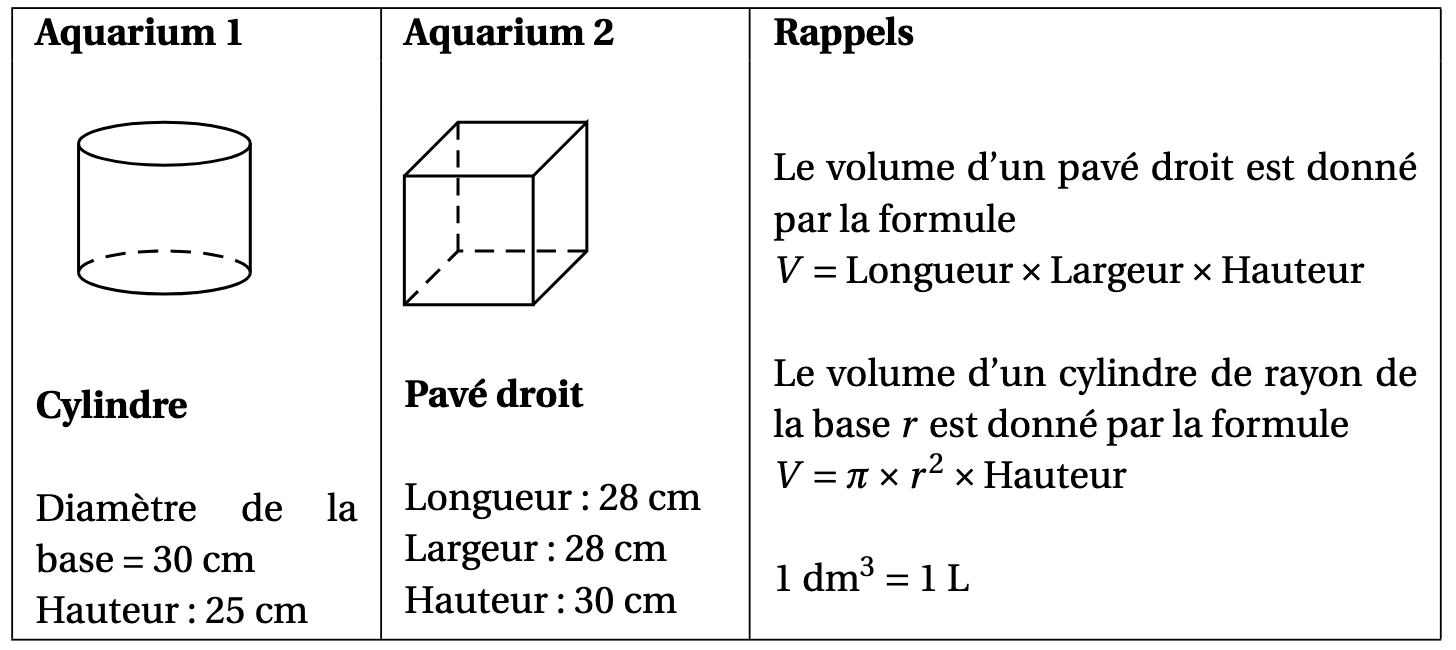
\includegraphics[scale=.65]{Tableau}
\end{center}


\end{enumerate}



\subsection*{Exercice 3,- 5 points}  %= 2+3

On considère le cube suivant, où $EF = 2$ cm. \begin{enumerate}
\item Calculer la longueur $AC$.
\item Calculer la longueur $FC$.
\end{enumerate}
\begin{center}
\includegraphics[scale=.5]{Exo3}\end{center}





 	\end{document}
